\documentclass[10pt]{standalone}
\usepackage{tikz}

% TikZ libraries `calc` needed now to tweak bracket.
\usetikzlibrary{backgrounds,fit,decorations.pathreplacing,calc}
% Dirac Kets
\newcommand{\ketone}[1]{\ensuremath{\left|#1\right\rangle^{\otimes nd}}}

\newcommand{\kettwo}[1]{\ensuremath{\left|#1\right\rangle^{\otimes n_0}}}

\newcommand{\ket}[1]{\ensuremath{\left|#1\right\rangle}}

\begin{document}
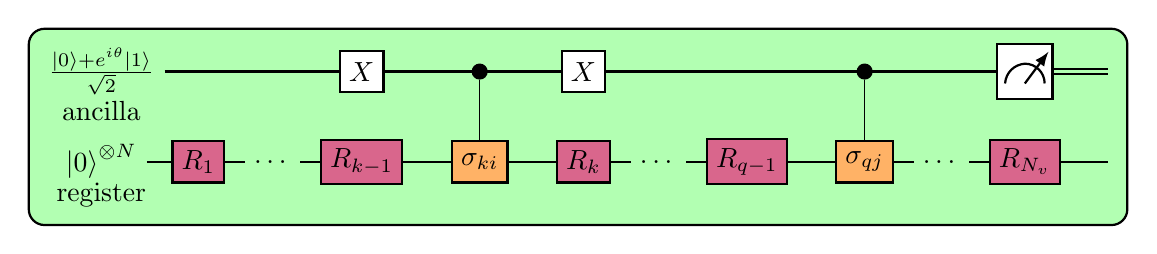
\begin{tikzpicture}[thick]
	% `phase' is used for controlled phase gates (dots).
	% `surround' is used for the background box.
	\tikzstyle{operator} = [draw,fill=white,minimum size=1.5em] 
	\tikzstyle{Roperator} = [draw,fill=purple!60!white,minimum size=1.5em] 
	\tikzstyle{Poperator} = [draw,fill=orange!60!white,minimum size=1.5em] 
	\tikzstyle{phase} = [draw,fill,shape=circle,minimum size=5pt,inner sep=0pt]
	\tikzstyle{surround} = [fill=green!30,thick,draw=black,rounded corners=2mm]
	\tikzstyle{blank} = [fill=green!30]
	%\tikzset{oldmeter/.append style={draw, inner sep=10, rectangle, font=\vphantom{A}, minimum width=30, line width=.8, path picture={\draw[black] ([shift={(.1,.3)}]path picture bounding box.south west) to[bend left=50] ([shift={(-.1,.3)}]path picture bounding box.south east);\draw[black,-latex] ([shift={(0,.1)}]path picture bounding box.south) -- ([shift={(.3,-.1)}]path picture bounding box.north);}}}
	 \tikzset{meter/.append style={draw, fill=white, inner sep=10, rectangle, minimum width=10pt,
	 path picture={\draw[black] (
 	[shift={(.1,.2)}]path picture bounding box.south west) to[bend left=40] %offset from bottom left corner
	([shift={(0,.1)}]path picture bounding box.center) to [bend left = 45] %To just offset from center
	([shift={(-.1,.2)}]path picture bounding box.south east) %To offset from bottom right of box
	;\draw[black,-latex] ([shift={(0,.2)}]path picture bounding box.south) -- ([shift={(.3,-.1)}]path picture bounding box.north);}]}} % Draw the arrow
	%
	\matrix[row sep=0.4cm, column sep=0.6cm] (circuit) {
	% First row.
		\node (q10) {$\frac{\ket 0 + e^{i\theta}\ket 1}{\sqrt 2}$}; &[-0.5cm]
		\coordinate (q12);&
		\coordinate (q13);&	
		\node[operator] (q14) {\ensuremath{X}}; &
		\node[phase] (q15) {};&
		\node[operator] (q16) {\ensuremath{X}}; &
		\coordinate (q17);&
		\coordinate (q18);&
		\node[phase] (q19) {};&
		\coordinate (q110);&
		\node[meter] (meter1) {};&
		\coordinate (end1); \\
	
		% Second row.
		\node (q20) {$\ket{0}^{\otimes N}$}; &
		\node[Roperator] (q22) {\ensuremath{R_1}}; & 
		\coordinate (q23);&
		\node[Roperator] (q24) {\ensuremath{R_{k-1}}}; & 
		\node[Poperator] (q25) {\ensuremath{\sigma_{ki}}}; & 
		\node[Roperator] (q26) {\ensuremath{R_{k}}}; & 
		\coordinate (q27);&
		\node[Roperator] (q28) {\ensuremath{R_{q-1}}}; & 
		\node[Poperator] (q29) {\ensuremath{\sigma_{qj}}}; & 
		\coordinate (q210);&
		\node[Roperator] (q211) {\ensuremath{R_{N_v}}}; &
		\coordinate (end2);\\
		};
	\node at ([yshift=-2pt] q10.south) (anc) {ancilla};
	\node at ([yshift=-2pt] q20.south) (reg) {register};
	% Draw bracket on right with resultant state.
		%\node[rectangle, draw, fill=white, minimum width = 1.5em, minimum height = 1.65cm][fit = (q17) (q27)] (box) {};
		%\node[align=center] at (box.center){A};
	\begin{pgfonlayer}{background}
		% Draw background box.
		\node at([yshift=-1.6em]end2) (corner) {};
		\node[surround] (background) [fit = (q10) (corner)] {};
		% Draw lines.
		\draw[thick] (q10) -- (meter1)  (q20) -- (end2) ;
		%\draw[thick] ([yshift=-5pt]5.5, 0.6725) -- ([yshift=-1pt]end1) ;
		%\draw[thick] ([yshift=-5pt]5.5, 0.740) -- ([yshift=1pt]end1) ;
		\draw[thick] ([yshift=1pt] meter1 |- 5.5, 1 |- end1) -- ([yshift=1pt]end1) ;
		\draw[thick] ([yshift=-1pt] meter1 |- 5.5, 1 |- end1) -- ([yshift=-1pt]end1) ;
		\draw (q15) -- (q25) ;
		\draw (q19) -- (q29) ;
		\node[blank] at (q23) (background) {\ldots};
		\node[blank] at (q27) (background) {\ldots};
		\node[blank] at (q210) (background) {\ldots};
		%\node at ([yshift=-1.5em]q210) (psi4) {\ket{\ensuremath{\psi_4}}};
		%\draw[->, >=stealth] (q111) -- (psi4);
	\end{pgfonlayer}
%
\end{tikzpicture}
\end{document}
